

\chapter{Regression and Reconstruction on \textit{d}-dimensional Cartesian Product Graphs}

\lhead{Chapter 6. \emph{Regression and Reconstruction on \textit{d}-dimensional Product Graphs}}

\label{chap:nd_gsp}

In this chapter we extend the methods developed in the previous two chapters, that is Graph Signal Reconstruction (GSR), Kernel Graph Regression (KGR) and Regression with Network Cohesion (RNC), to graphs which are the Cartesian product of three or more factor graphs. 

\begin{itemize}
    \item Summarise chapter aims and output
    \item Give motivation for MWGSP
\end{itemize}


\section{\textit{d}-dimensional graph signal processing}

In \cref{sec:graph_products_defined} we gave the general definition of a product between two graphs and highlighted four standard examples, namely the Cartesian, direct, strong and lexicographic products. Each of these product types can be straightforwardly extended to more than two factor graphs by applying their respective definition recursively. For example, consider the Cartesian product between graphs $\mathcal{G}_A = \{\mathcal{V}_A, \mathcal{E}_A\}$, $\mathcal{G}_B = \{\mathcal{V}_B, \mathcal{E}_B\}$ and $\mathcal{G}_C = \{\mathcal{V}_C, \mathcal{E}_C\}$ where $|\mathcal{V}_A| = A$, $|\mathcal{V}_B| = B$ and $|\mathcal{V}_C| = C$. This can be written as 

\begin{equation}
    \mathcal{G} \; = \; \mathcal{G}_A \, \square \; \mathcal{G}_B \, \square \; \mathcal{G}_C \; = \; \{\mathcal{V}, \, \mathcal{E}\}
\end{equation}

The new vertex set, $\mathcal{V}$, is given by the Cartesian product of the individual vertex sets. 

\begin{equation}
    \mathcal{V} = \mathcal{V}_A \times \mathcal{V}_B \times \mathcal{V}_C = \{(a, \, b, \, c) \in \mathbb{N}^3 \, | \, a \leq A, \; b \leq B, \text{and} \;  c \leq C\}
\end{equation}

The new edge set, $\mathcal{E}$, is given by recursively applying conditions 1 and 7 from, \cref{sec:graph_products_defined} to the new node set. In particular, any two nodes $(a, \, b, \, c)$ and $(a', b', c')$ are connected in $\mathcal{E}$ if they satisfy any of the following three conditions. 

\vspace{0.5cm}

\begin{table}[h]
    \def\arraystretch{1.5}
    \centering
    \begin{tabular}{lclclc}
        1. & $[a, \, a'] \in \mathcal{E}_A$    & and & $b = b'$  & and & $c = c'$             \\
        2. & $a = a'$    & and & $[b, \, b'] \in \mathcal{E}_B$   & and & $c = c'$             \\
        3. & $a = a'$    & and & $b = b'$  & and & $[c, \, c'] \in \mathcal{E}_C$              \\
    \end{tabular}
\end{table}


\begin{figure}[t]
    \begin{center}
        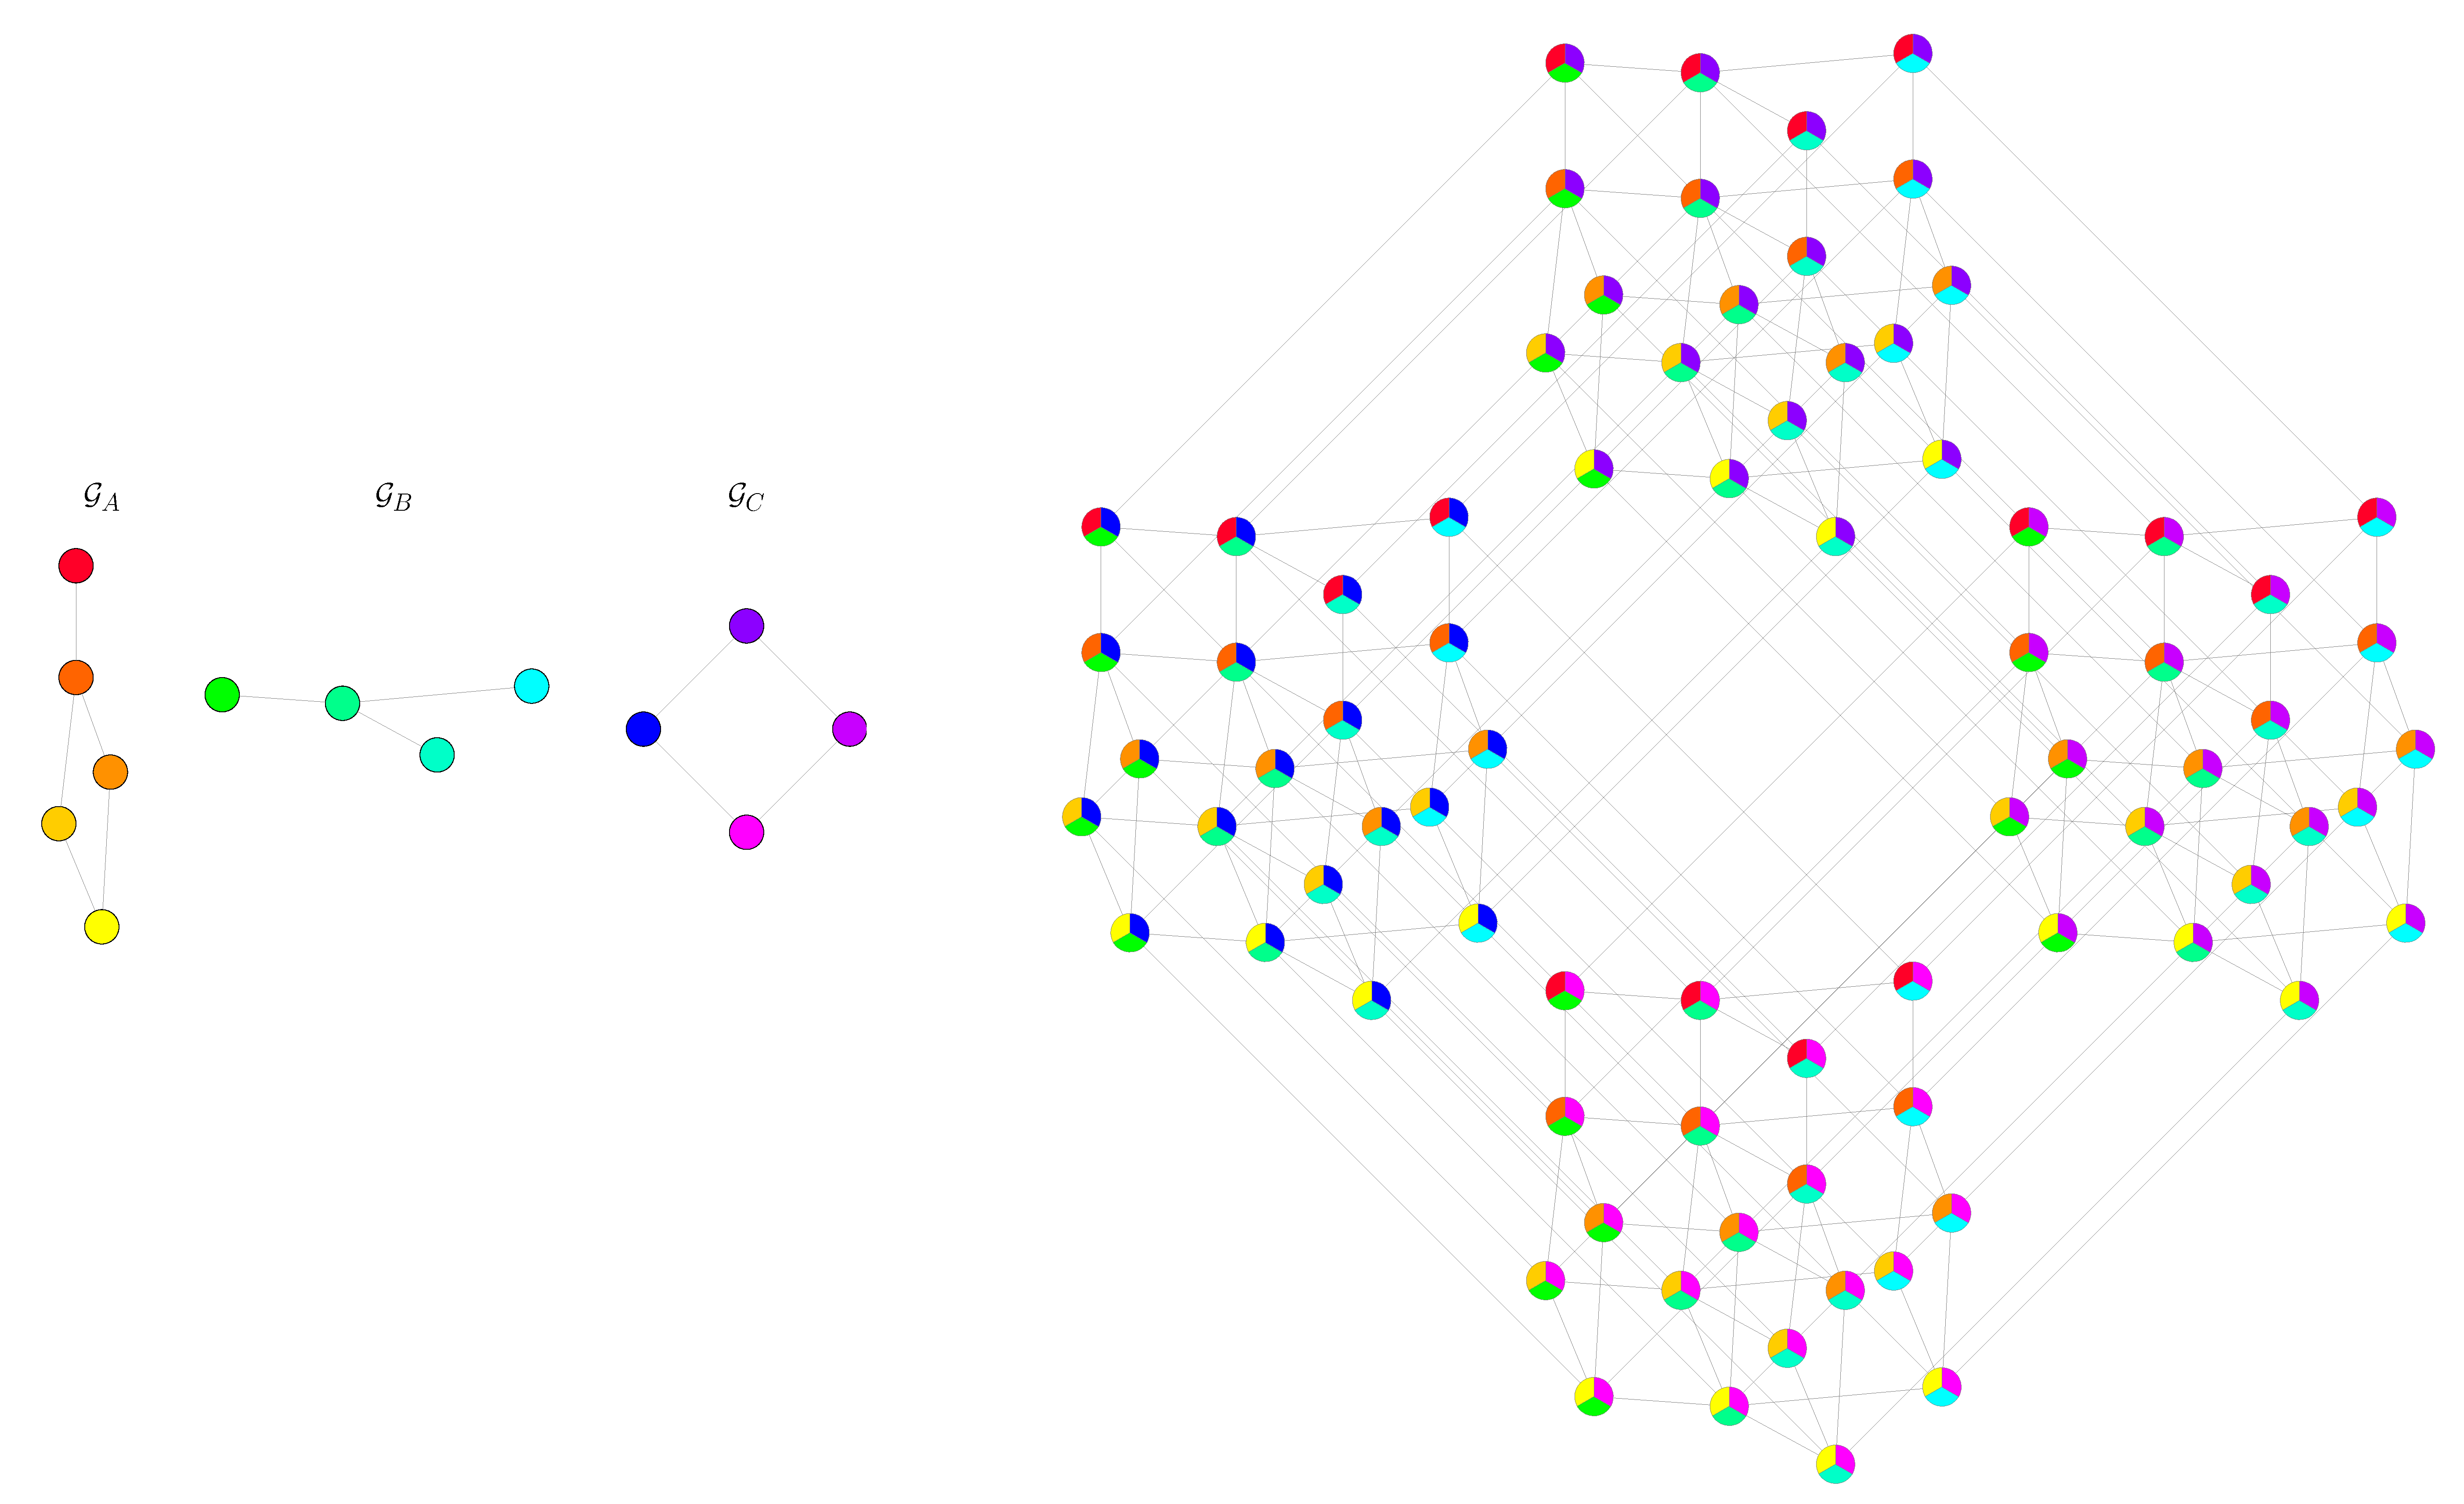
\includegraphics[width=\linewidth]{Figures/3D_CPG.pdf}
    \end{center}
    \caption[Graphical depiction of a 3D Cartesian product graph]{Graphical depiction of a 3D Cartesian product graph}
    \label{fig:3D_CPG}
\end{figure}

\Cref{fig:3D_CPG} gives a visual representation of a Cartesian product graph formed from three simple factor graphs. Notice that the size of the new vertex and edge set both grow very quickly. In particular, 

$$
|\mathcal{V}| = |\mathcal{V}_A| |\mathcal{V}_B| |\mathcal{V}_C| \aand |\mathcal{E}| =  |\mathcal{E}_A| |\mathcal{V}_B| |\mathcal{V}_C| + |\mathcal{V}_A| |\mathcal{E}_B| |\mathcal{V}_C| + |\mathcal{V}_A| |\mathcal{V}_B| |\mathcal{E}_C|
$$

Happily, the adjacency matrix of a Cartesian product graph $\A$ has a simple representation in terms of the factor adjacency matrices (here $\A_A$, $\A_B$ and $\A_C$). 

\begin{align}
    \A &= \A_A \oplus \A_B \oplus \A_C \notag \\
    &= \A_A \otimes \I_B \otimes \I_C  + \I_A \otimes \A_B \otimes \I_C + \I_A \otimes \I_B \otimes \A_C
\end{align}

In general, we can consider the Cartesian product of $d$ factor graphs with adjacency matrices denoted as $\A^{(1)} \in \R^{N_1 \times N_2}, \A^{(2)} \in \R^{N_2 \times N_2}, \dots \A^{(d)} \in \R^{N_d \times N_d}$. The full adjacency matrix will have size $N \times N$, where $N = \prod N_i$, and is given by  

\begin{alignat}{4}
    \A = \A^{(1)} & \oplus \A^{(2)} & \oplus \;\; ... \;\; & \oplus \A^{(d)} \notag \\[0.1cm]
    = \A^{(1)} & \otimes \I_{N_2} & \otimes \;\; ... \;\; & \otimes \I_{N_d} +  \notag \\[0.1cm]
    \I_{N_1} & \otimes \A^{(2)} & \otimes \;\; ... \;\; & \otimes \I_{N_d} + \;\; \ldots \;\; +  \notag \\[0.1cm]
    \I_{N_1} & \otimes \I_{N_2} & \otimes \;\; ... \;\; & \otimes \A^{(d)}  
\end{alignat}
    
This can be written compactly as 

\begin{equation}
    \A = \bigoplus_{i=1}^d  \A^{(i)}
\end{equation}

Similarly, the Laplacian of the product graph, $\LL$, can be written as the Kronecker sum of the individual factor graph Laplacians $\LL^{(i)}$. 

\begin{equation}
    \LL = \bigoplus_{i=1}^d  \LL^{(i)}
\end{equation}

We can perform eigendecomposition on each of the individual graph Laplacians as follows. 

\begin{equation}
    \LL^{(i)} = \U^{\,(i)} \LAM^{(i)} (\U^{\,(i)})^\top
\end{equation}

\noindent where $ \U^{(i)}$ is an orthogonal matrix such that each column is an eigenvector of $\LL^{(i)}$, and $\LAM^{(i)}$ is a diagonal matrix containing the corresponding eigenvalues, which are typically listed in ascending order. Given this, the Laplacian of the product graph can be decomposed as follows. 

\begin{align}
    \LL &= \bigoplus_{i=1}^d \U^{\,(i)} \LAM^{(i)} (\U^{\,(i)})^\top \notag \\[0.2cm]
    &= \left( \bigotimes_{i=1}^d  \U^{\,(i)} \right) \left(\bigoplus_{i=1}^d \LAM^{(i)} \right) \left(\bigotimes_{i=1}^d  \U^{\,(i)} \right)^\top \notag \\[0.2cm]
    &= \U \LAM \U^\top 
\end{align}

\noindent where 

$$
\U =  \bigotimes_{i=1}^d  \U^{\,(i)} , \quad \text{and} \quad \LAM =  \bigoplus_{i=1}^d \LAM^{(i)}
$$

Here, we have used the notation $\bigotimes_{i=1}^d  \U^{\,(i)}$ to denote the chained Kronecker product of matrices $\{\U^{\,(i)}  \}$. 

A graph signal $\y$ existing on the nodes of a $d$-dimensional product graph can be represented as either a $d$-dimensional array (tensor) of shape $(N_1 \times N_2 \times ... \times N_d)$, or a vector of length $N = \prod_{i=1}^d N_i$. In the next section we discuss these two representations and how to convert between them in practice. For now, assume the signal is a length-$N$ vector. We can define its Graph Fourier Transform (GFT) and the corresponding inverse (IGFT) as follows. 

\begin{alignat}{2}
\label{eq:gft}
    \text{GFT}(\y) & = \U^\top \y && = \Big(  \bigotimes_{i=1}^d  \U^{\,(i)} \Big)^\top \y \\
\label{eq:igft}
    \text{IGFT}(\y) & = \U \y && = \Big(  \bigotimes_{i=1}^d  \U^{\,(i)} \Big) \; \y 
\end{alignat}

Given these definitions, we can naturally define the concept of a graph filter. A graph filter acts on a signal $\y$ by scaling the amplitude of its spectral components according to some function of the corresponding frequency $g(\lambda; \beta)$. Most commonly, a low-pass graph filter, such as one provided in table \ref{tab:filters}, is used, such that the high frequency components of a signal are attenuated. 



\section{Fast computation with \textit{d}-dimensional Kronecker products}

Hello

\section{Signal reconstruction}

Hello

\section{Kernel Graph Regression}

Hello

\section{Regression with Network Cohesion}

Ahhhh

\section{Regression with Network Cohesion}